\documentclass{article}
\usepackage{graphicx}

\begin{document}

\begin{center}



\includegraphics[width=3cm]{/storage/emulated/0/Pictures/Screenshots/IMG_20260310_120019.jpg}


\vspace{0.5cm}

{\huge GATE CS 2010 - Question 9}

\vspace{0.3cm}

Keshava Reddy V

ID: COMETFWC054

\end{center}

\section*{Question}

The Boolean expression for the output $F$ of the multiplexer is to be determined.

The circuit is a $4:1$ multiplexer with select lines $P$ and $Q$.

Inputs:

$I_0 = R$

$I_1 = \overline{R}$

$I_2 = \overline{R}$

$I_3 = R$

\section*{Analysis}

Select lines are $P$ and $Q$.

\begin{center}
\begin{tabular}{|c|c|c|}
\hline
$P$ & $Q$ & Output \\
\hline
0 & 0 & $R$ \\
0 & 1 & $\overline{R}$ \\
1 & 0 & $\overline{R}$ \\
1 & 1 & $R$ \\
\hline
\end{tabular}
\end{center}

After simplification,

$F = P \oplus Q \oplus R$

\section*{Python Code}

\begin{verbatim}
import numpy as np
import matplotlib.pyplot as plt

P = np.array([0,0,0,0,1,1,1,1])
Q = np.array([0,0,1,1,0,0,1,1])
R = np.array([0,1,0,1,0,1,0,1])

F = P ^ Q ^ R

print("P Q R | F")
for i in range(8):
    print(P[i],Q[i],R[i],"|",F[i])

x = np.arange(8)
plt.stem(x,F)

plt.savefig("graph.png")
plt.show()
\end{verbatim}

\section*{Graph}

\begin{center}

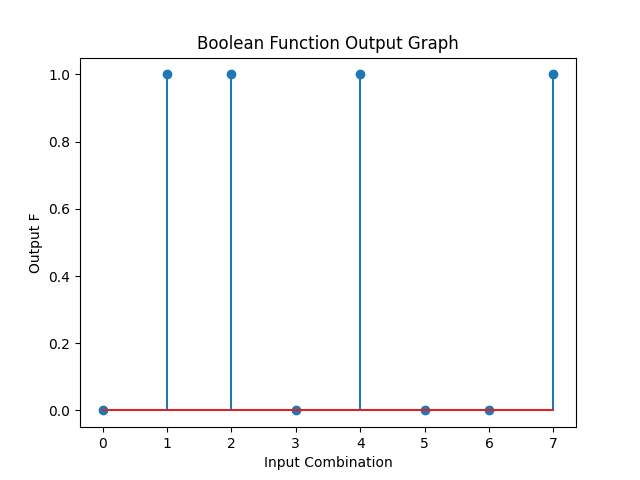
\includegraphics[width=10cm]{graph.png}

\end{center}

\section*{Conclusion}

The simplified Boolean expression for the multiplexer output is

$F = P \oplus Q \oplus R$.

\end{document}
